
MQAM system is a complex block of code that simulates the modulation, transmission and demodulation of an optical signal using M-QAM modulation.
	
It is composed of four blocks: a transmitter, a receiver, a communication channel and a block that performs a Bit Error Rate (BER) measurement. The schematic representation of the system is presented in figure \ref{MQAM_system_block_diagram}.

\begin{figure}
	\centering
	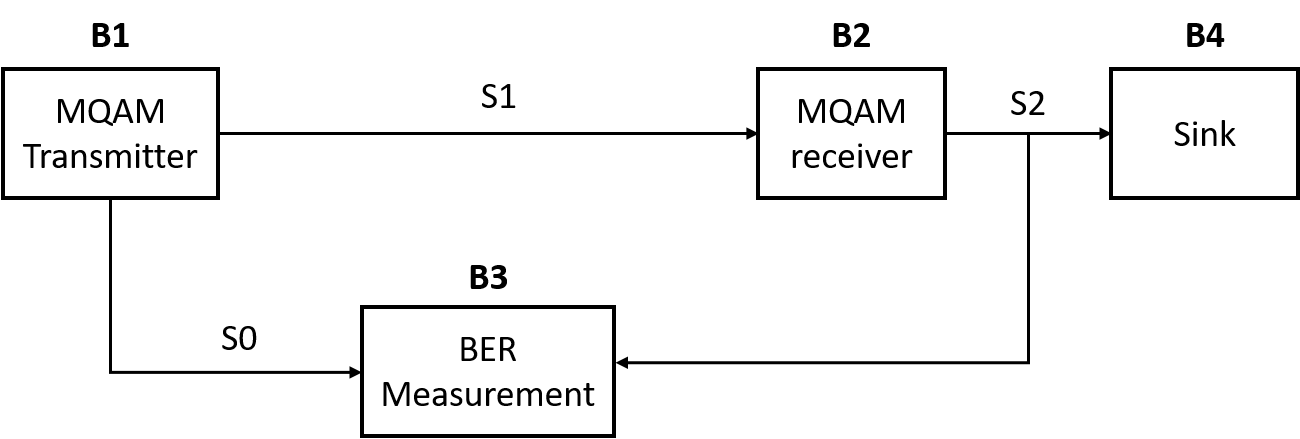
\includegraphics[width=0.8\textwidth]{./figures/MQAM_system_block_diagram}
	\caption{Schematic representation of the MQAM system.}\label{MQAM_system_block_diagram}
\end{figure}

\subsection*{MQAM transmitter}

A complete description of the MQAM transmitter either block by block or as a whole can be found in the \textit{lib} repository. 

This block generates one or two optical signals. It also generates a binary signal that is used to perform a BER measurement.

\subsection*{MQAM receiver (homodyne receiver)}

A complete description of the MQAM transmitter either block by block or as a whole can be found in the \textit{lib} repository.

The MQAM receiver is a homodyne receiver. It accepts one input optical signal and outputs a binary signal. It performs the M-QAM demodulation of the input signal.

\subsection*{BER measurement}

In this section we present the results of the BER measurement for the MQAM system.

\begin{figure}
	\centering
	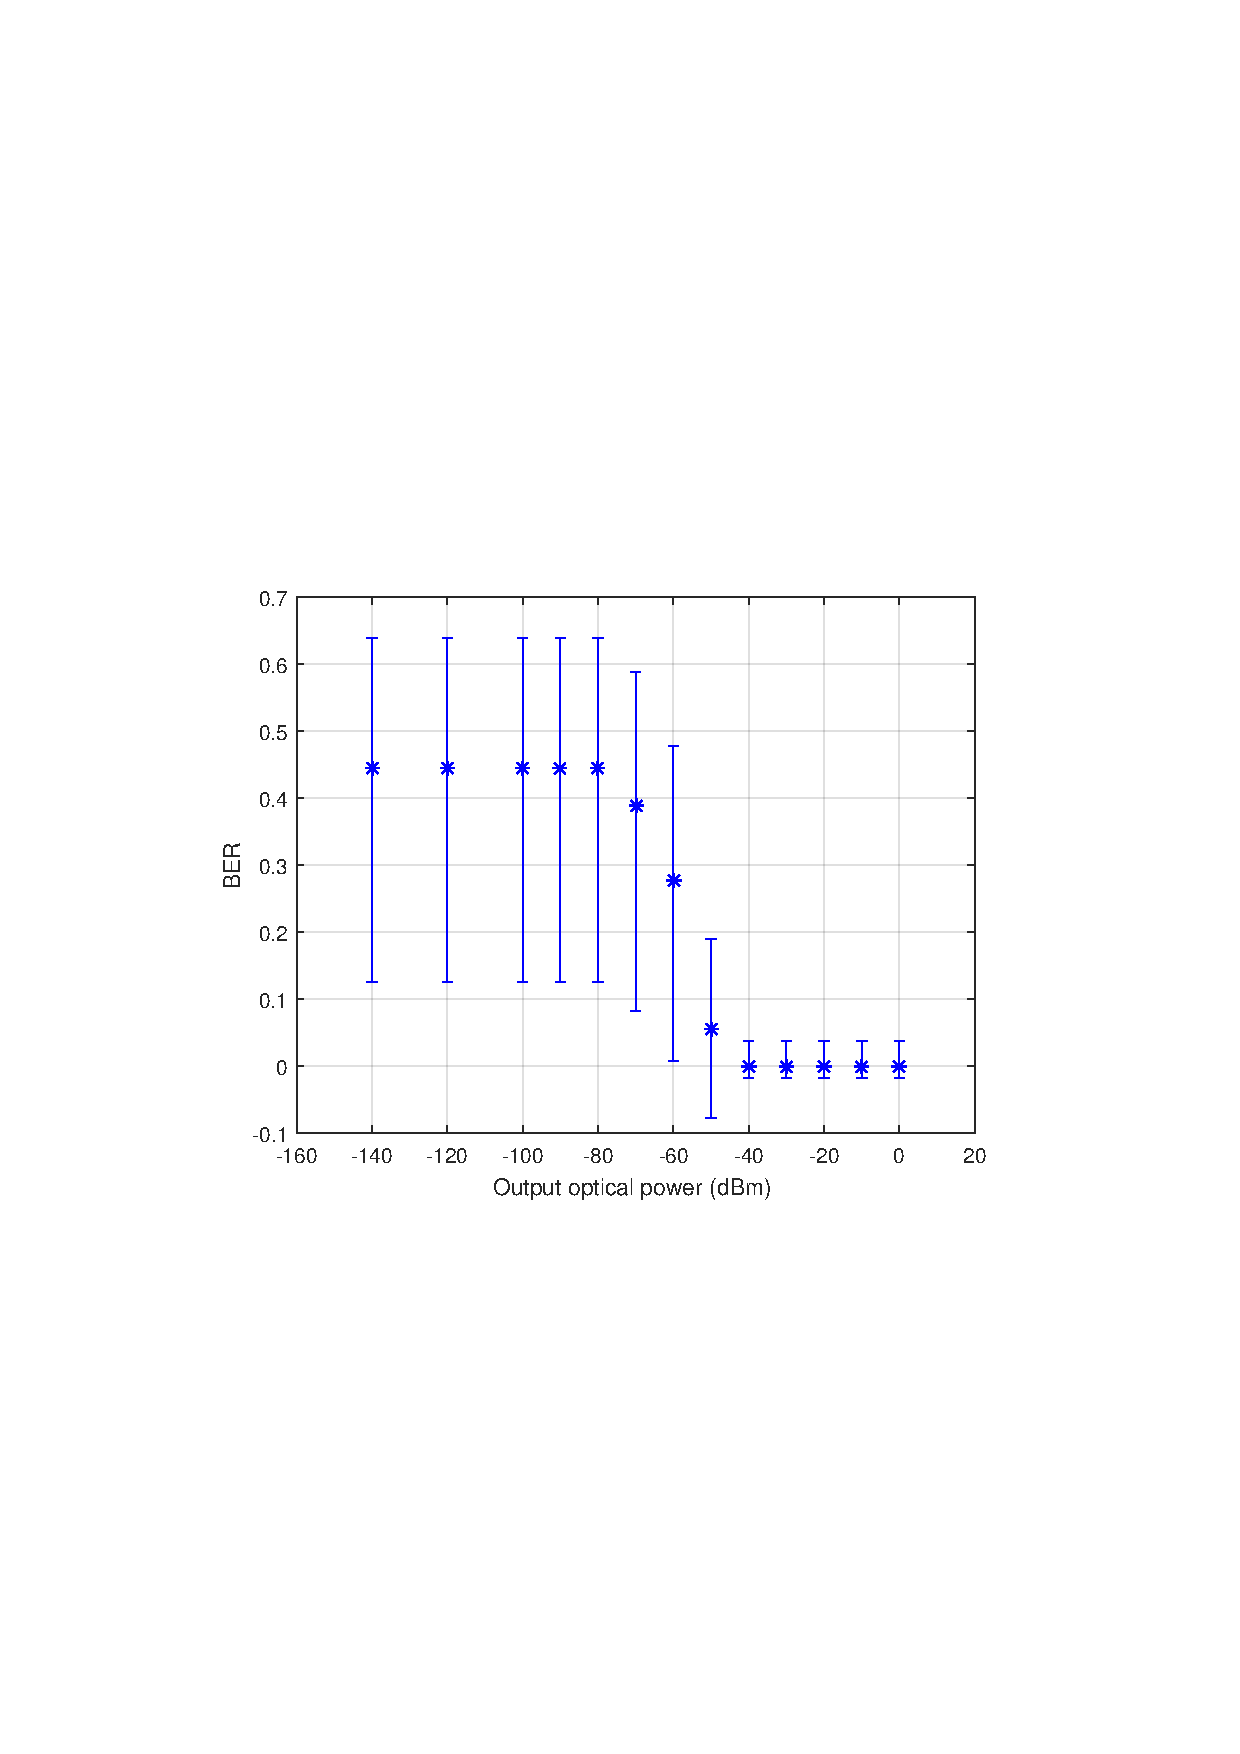
\includegraphics[width=\textwidth]{./figures/BER_LO0_Noise20}
	\caption{BER measurement for a local oscillator power of 0 dBm and a noise level of 20}\label{fig:BER20}
\end{figure}

\begin{figure}
	\centering
	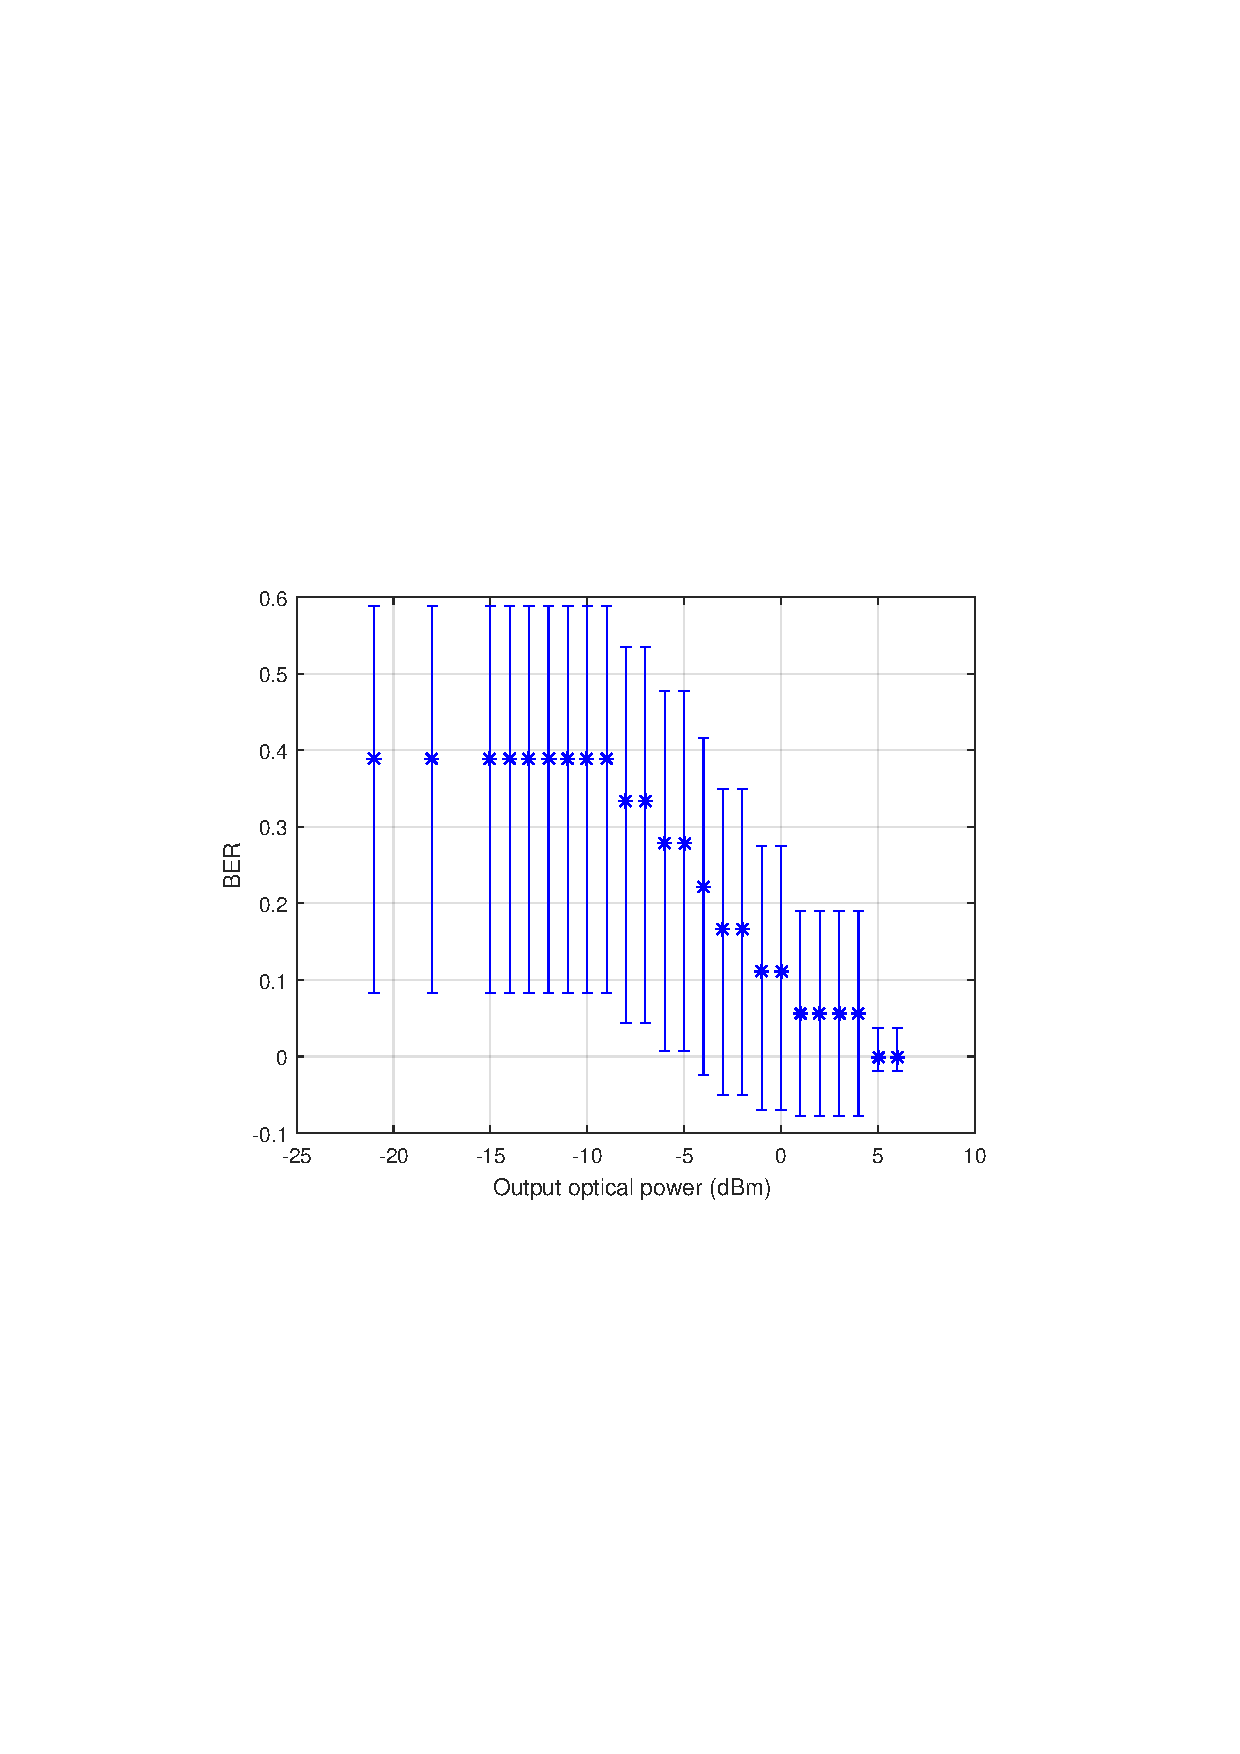
\includegraphics[width=\textwidth]{./figures/BER_LO0_Noise10000}
	\caption{BER measurement for a local oscillator power of 0 dBm and a noise level of 10000}\label{fig:BER10000}
\end{figure}

\subsection*{Input parameters}

The input parameters of the system are the ones from the MQAM transmitter plus the ones from the MQAM receiver.

